\documentclass{beamer}
 
\usepackage[utf8]{inputenc}
\usepackage{amsmath}
\usepackage{amssymb}
\renewcommand\mathfamilydefault{\rmdefault}

 
 
%Information to be included in the title page:
\title{More Combinatorics}
\author{Ben Kettle}
\date{22 Jan 2020}
 
\begin{document}
 
\frame{\titlepage}

\begin{frame}{Summary of Combinatorics}
    Over the last two weeks, we covered:
    \begin{itemize}
        \item Subsets
        \item Permutations
        \item Bijections
        \item Division Rule
        \item Combinations
    \end{itemize}
    There's a very brief summary of all of these on your handout---are there any other questions about these?
\end{frame}

\begin{frame}{Practice}
    To get into the mood for combinatorics, I made some exercises for you guys to do. You can work on them alone or in groups, and ask if you have questions!
\end{frame}

\begin{frame}{Intro to Probability}
    Based on the numbers you guys calculated for these, which hand do you think is preferred by poker players? \vspace{2mm}
    
    The hands with fewer possibilities! These hands are rarer, and thus less likely to occur. In other words, on a certain deal, the \alert{probability} of a player receiving one of these hands is low.
\end{frame}

\begin{frame}{Coin Flipping}
    Let's look at your coin flipping results. Add up the number of heads and the number of tails for each of your flips. \vspace{2mm}
    
    \visible<2->{I'm sure you guys know that the probability of getting heads (or tails) on a coin flip is $\frac{1}{2}$. So let's see how the experimental results line up with that.}
    
    \visible<3->{When the number of coin flips is low, the results may not seem to reflect the probability. However, as the number of trials increases, the experimental results should represent the theoretical probability more and more closely.}
\end{frame}

\begin{frame}{A Game Show Example}
    \begin{figure}
        \centering
        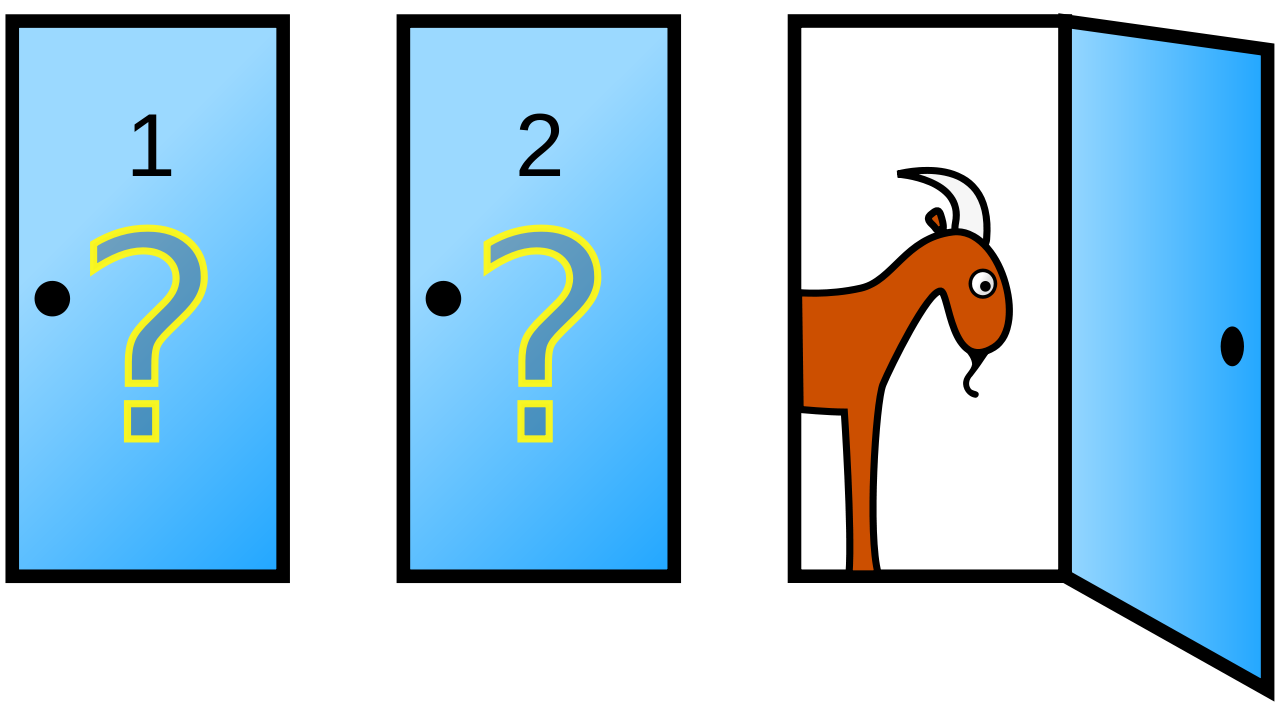
\includegraphics[scale=.06]{montyhalldoors.png}
    \end{figure}
    In the 1970's, there was a game show called \textit{Let's Make a Deal}. On the show, contestants were faced with 3 closed doors: one had a car behind it, and the other two had goats behind them. In the show, there are three stages:
    
    \begin{enumerate}
        \item The contestant chooses a door.
        \item The host then opens one of the doors \textit{without the prize}, revealing a goat. 
        \item The contestant is given the opportunity to switch doors to the remaining unrevealed door.
    \end{enumerate}
    Should the contestant switch doors? Let's find out.
\end{frame}

\begin{frame}{Let's Make a Deal}
    To make sure you guys understand the premise, let's do an example. 
\end{frame}

\begin{frame}{Try it!}
    In your groups, try it out. Use the table on the back of one group member's handout to keep track of the results, and have everyone in your group be the "host". Here are the steps of the game again:
    
    \begin{enumerate}
        \setcounter{enumi}{-1}
        \item The host randomly chooses one door as a winner---the other two have goats behind them.
        \item The contestant chooses a door.
        \item The host then opens one of the doors \textit{without the prize}, revealing a goat. 
        \item The contestant is given the opportunity to switch doors to the remaining unrevealed door.
    \end{enumerate}
    
    Make sure your group tries both switching to the other door and staying with the original door.
    
\end{frame}

\begin{frame}{Solving Probability Problems}

Clearly, probability can be unintuitive---I have a hard time wrapping my head all the way around this result. Luckily, though, we don't have to rely on only our intuition to solve these. \vspace{5mm}

To solve these probability problems, we define what we call the \alert{4-step method}, which helps us turn these into concrete math problems:

\begin{enumerate}
    \item Find the sample space
    \item Define events of interest
    \item Determine outcome probabilities
    \item Compute event probabilities
\end{enumerate}

We'll go through these step-by-step to understand this problem and determine the probabilities of winning. To simplify the problem, we'll only consider the probability of \textit{winning by switching}.
\end{frame}

\begin{frame}{Step 1: Determine Sample Space}
    All this step is asking us to do is find some way of representing the outcomes of the experiment. It's almost always good to draw at least some part of a tree, and for this problem it's not to bad to draw the whole thing. We'll base it on the same steps as above:
    \begin{enumerate}
        \item The door the host chooses as correct
        \item The door the contestant chooses
        \item The revealed door
    \end{enumerate}\vspace{5mm}
    \visible<2->{
    To simplify the way we discuss the problem, we'll define each chain through the path with a sequence:
    \begin{center}
        (door concealing prize, door initially chosen, door opened by host)
    \end{center}}
\end{frame}

\begin{frame}{The Tree}
    \begin{figure}
        \centering
        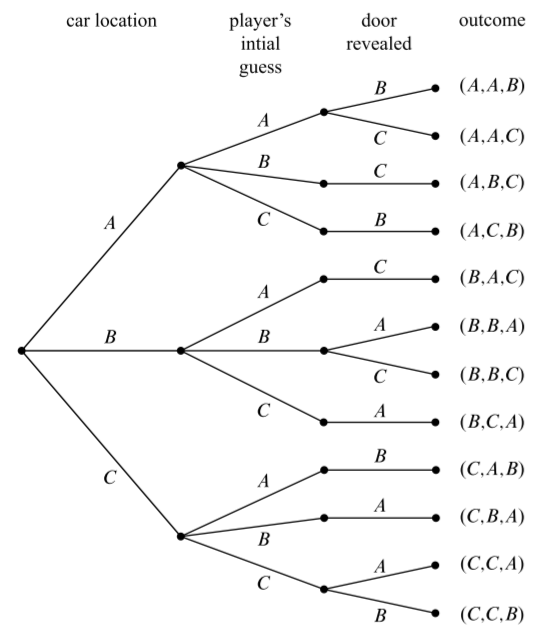
\includegraphics[scale=.5]{montyhalloutcomes.png}
        \caption{The tree diagram for \textit{Let's Make a Deal}, including the outcomes.}
        \label{fig:montyhalloutcomes}
    \end{figure}
\end{frame}

\begin{frame}{Step 1: Determine Sample Space}
    Using this tree to help us, we can see that the sample space is 
    
    \[ S=\left\{\begin{array}{l}
{(A, A, B), (A, A, C), (A, B, C), (A, C, B),} \\ {(B, A, C),(B, B, A), (B, B, C),(B, C, A)}, \\{(C, A, B),(C, B, A),(C, C, A),(C, C, B)}
\end{array}\right\} \]
\end{frame}

\begin{frame}{Step 2: Define Events of Interest}
    We have this nice list of outcomes, but we don't actually care about what the outcome specifically is. Instead, what we want is the probability of an event, such as "the host reveals door B". 
    
    For example, the set of outcomes specified by the event "the prize is behind door $C$" is:
    
    \[ \{(C, A, B),(C, B, A),(C, C, A),(C, C, B)\}\]
    
    \begin{itemize}
        \item What is the set of outcomes for the event we really care about, that "the player wins by switching?"
    \end{itemize}
    \vspace{2mm}
    \visible<2->{\alert{ These are all the cases where the player did not initially chose the correct door.
    \[ \{(A,B,C),(A,C,B),(B,A,C),(B,C,A),(C,A,B),(C,B,A)\}\]
    
    Let's update our tree to reflect this.
    }}
\end{frame}

\begin{frame}{The Tree: Switch Wins}
    \begin{figure}
        \centering
        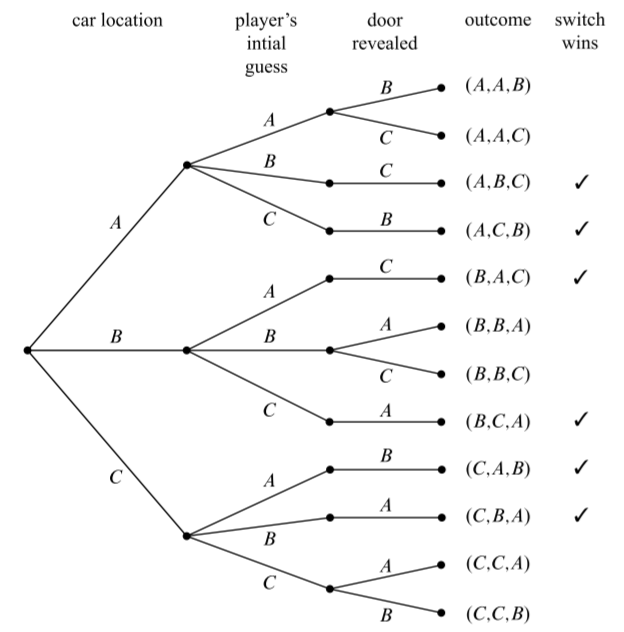
\includegraphics[scale=.5]{montyhalloutcomes2.png}
        \caption{The tree diagram for \textit{Let's Make a Deal}, including the cases where switching wins.}
        \label{fig:montyhalloutcomes2}
    \end{figure}
\end{frame}

\begin{frame}{Step 3: Determine Outcome Probabilities}
You may have noticed that on our tree, switching wins in exactly half of the cases. However, this \textbf{does not} mean that the probability of winning by switching is $\frac{1}{2}$. This is because each outcome has a different \alert{outcome probability}.\vspace{2mm}

To calculate these outcome probabilities, we first assign the \textit{edge} probabilities, and then multiply along each to determine each outcome probability. \vspace{2mm}

Let's go through and assign the edge probabilities to our tree, then find the outcome probabilities. \vspace{2mm}

\visible<2->{In doing this, we've defined a function mapping an outcome to its probability. This function is usually called \textbf{Pr}. For example, $Pr[(A,A,B)]=\frac{1}{18}$}. We'll see this throughout probability.
\end{frame}

\begin{frame}{The Tree: Edge Probabilities}
    \begin{figure}
        \centering
        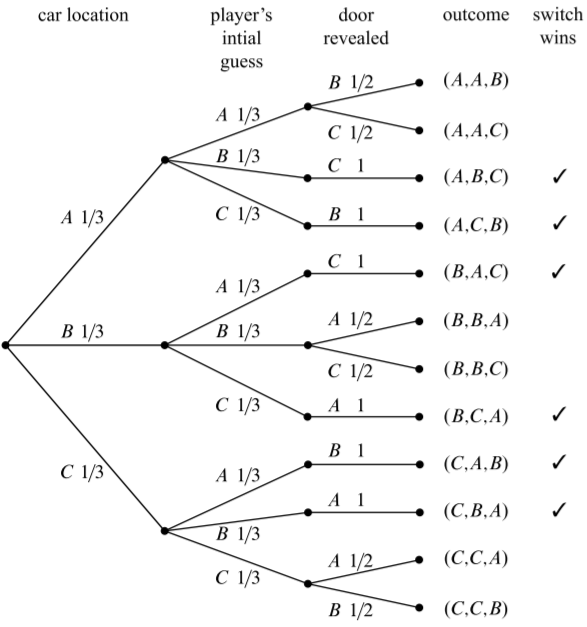
\includegraphics[scale=.5]{montyhalledgeprobs.png}
        \caption{The tree diagram for \textit{Let's Make a Deal}, including the probabilities along each edge.}
        \label{fig:montyhalledge}
    \end{figure}
\end{frame}

\begin{frame}{The Tree: Outcome Probabilities}
    \begin{figure}
        \centering
        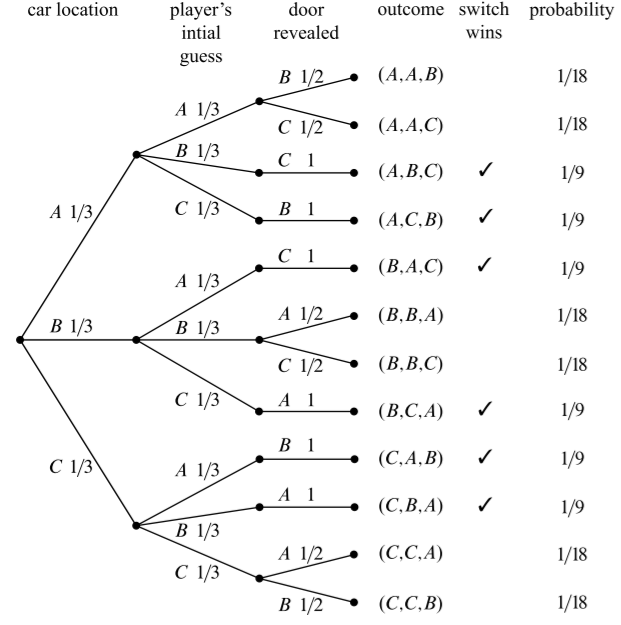
\includegraphics[scale=.5]{montyhalloutcomeprobs.png}
        \caption{The tree diagram for \textit{Let's Make a Deal}, including the probabilities of each outcome.}
        \label{fig:montyhalloutprob}
    \end{figure}
\end{frame}

\begin{frame}{Step 4: Compute Event Probabilities}
    Now that we have probabilities for each outcome, we can combine these to find an \alert{event probability}. As we saw earlier, if any outcome of the outcomes the event specifies occurs, the event happens.
    \begin{itemize}
        \item What is the probability of the event "the player wins by switching" then? \visible<2->{We can see that each of the outcomes specified by this event has probability $\frac{1}{9}$. Because any one of these events can occur, we can \textit{add} the individual probabilities. Thus, the probability of winning by switching is $\frac{2}{3}$, and the probability of winning by switching is 2/3, while the probability of winning by staying is its complement 1/3.}
    \end{itemize}
\end{frame}

\begin{frame}{Conclusion}
    So, we did the math behind the problem to figure out that it's better for the contestant to switch. Probabilities can often be confusing like this, so it's often good to follow this method to understand what's going on. And before you start, always make sure you fully understand the problem!
\end{frame}

\begin{frame}{Another Example: Strange Dice}
    Let's say you're at a bar getting some coffee, and someone sits down next to you and offers to make you a bet. He has 3 dice, and he wants to bet \$100 that he will roll higher than you will. \vspace{2mm}
    
    \visible<2->{But these are not normal dice. They have weird numbers on the sides: 
    
    \begin{figure}
        \centering
        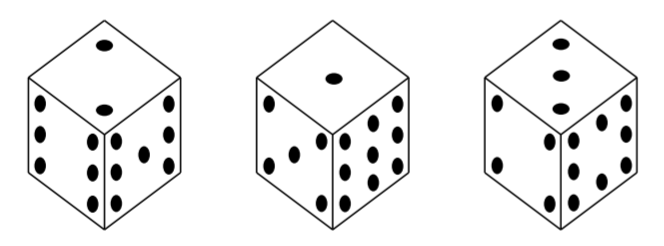
\includegraphics[scale=.5]{strangedice.png}
        \caption{The strange dice, $a$, $b$, and $c$ from left to right.}
    \end{figure}
    Would you take the deal? \vspace{2mm}}
\end{frame}

\begin{frame}{Strange Dice}
    He sees that you're hesitant, and offers a better offer: you can pick your die first, and he will have one of the remaining two. Now what do you think?
    
    \vspace{2mm}
    
    \visible<2->{In order to find out how to defeat this guy, you want to calculate the probability of winning for each pair of dice. This way, you'll know which die you should pick. Again, the sides of the dice:
    
    \begin{center}
        $a$: $\{2,2,6,6,7,7\}$, $b$: $\{1,1,5,5,9,9\}$, $c$: $\{3,3,4,4,8,8\}$
    \end{center} 
    
    In a group of 4ish, try to solve this! Apply the four-step method as we just did to find the best die to choose (if there is one!):
    \begin{enumerate}
        \item Find the sample space
        \item Define events of interest
        \item Determine outcome probabilities
        \item Compute event probabilities
    \end{enumerate}}
\end{frame}

\begin{frame}{The Tree: A vs B}
    \begin{figure}
        \centering
        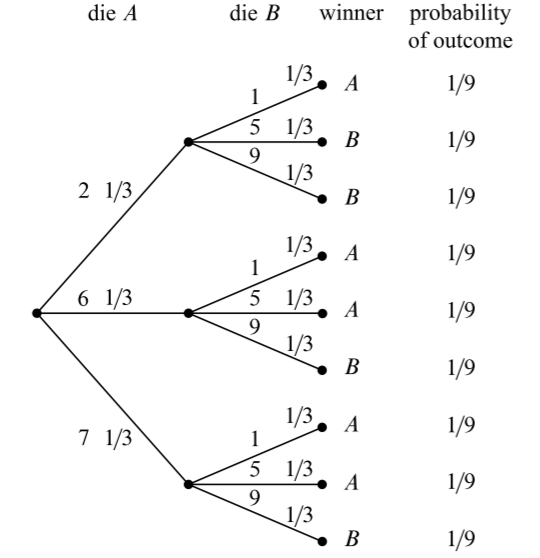
\includegraphics[scale=.5]{strangeavsb.png}
        \caption{The tree diagram for one roll of die $A$ vs die $B$. Adding up the winning outcomes, we can see that die $B$ wins with probability $5/9$.}
    \end{figure}
\end{frame}

\begin{frame}{The Tree: B vs C}
    \begin{figure}
        \centering
        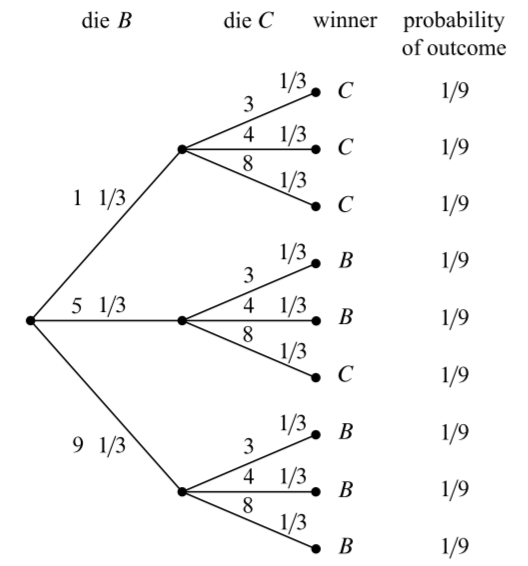
\includegraphics[scale=.5]{strangebvsc.png}
        \caption{The tree diagram for one roll of die $B$ vs die $C$. Adding up the winning outcomes, we can see that die $B$ wins with probability $5/9$.}
    \end{figure}
\end{frame}

\begin{frame}{The Tree: C vs A}
    \begin{figure}
        \centering
        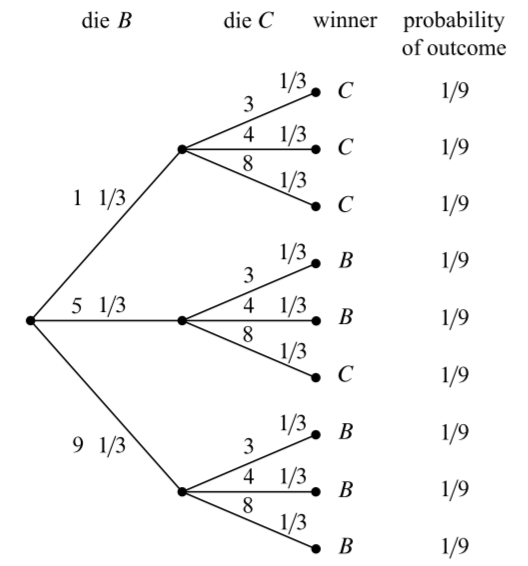
\includegraphics[scale=.5]{strangebvsc.png}
        \caption{The tree diagram for one roll of die $C$ vs die $A$. Adding up the winning outcomes, we can see that die $C$ wins with probability $5/9$.}
        \label{fig:my_label}
    \end{figure}
\end{frame}

\begin{frame}{Back to the Bet}
    So, we found that:
    \begin{itemize}
        \item $C$ beats $A$ with probability $5/9$
        \item $A$ beats $B$ with probability $5/9$
        \item $B$ beats $C$ with probability $5/9$
    \end{itemize}
    Again, probability can be unintuitive, so it's important to go through the concrete math behind it. In this case, there is no best die for you to pick! \vspace{2mm}
    
    That's because this property \textit{seems} like it should be transitive---if die $C$ is likely to be better than die $B$, and die $B$ is likely to be better than die $A$, then die $C$ should be better than die $A$, right? In this case, no! \vspace{2mm}
    
    And it gets even weirder. If you roll the dice twice instead, and take the sum, the order switches!
\end{frame}

\begin{frame}{Conditional Probabilities}
    Trees are useful, but we don't \textit{have} to use them every time. We can extract a few formulas from the tree that we can use to simplify problems in the future. \vspace{2mm}
    
    The first of these, and probably the most used, is called \alert{conditional probability}. That is, if we \textit{know} that one event happened, what is the probability that another event happens? \vspace{2mm}
\end{frame}

\begin{frame}{Conditional Probabilities: Example}
    Let's define $A_7$ as the event that die $A$ rolls a 7 and $B$ as the event that die $B$ wins. From multiplying along the path, we know that the probability of $A_7$ AND $B$ ($Pr(A_2 \cap B)$) is $1/9$.
    
    
    \begin{itemize}
        \item Look at your tree for the \textbf{$A$ vs $B$} case from the strange dice problem. What is the probability of event $B$, \alert{given} that A rolled a 7? In math terms, we want $Pr(B|A_7)$. \visible<2->{\alert{We can see that there is only one case with probability $1/9$ that event $B$ occurs given event $A_7$ occurs, so $Pr(B|A_7)=1/9$.}}
        \visible<3->{\item If $A_2$ is the event that $A$ rolls a 2, what is $Pr(B|A_2)$} \visible<4->{\alert{There are two cases here with probability $1/9$, so this is $2/9$.}}
    \end{itemize}
\end{frame}

\begin{frame}{Formalizing Conditional Probabilities}
    We can formalize this concept for any two events $A$ and $B$. \vspace{2mm}
    
    \textbf{Definition:} Conditional Probability \newline
    For any two events $A$ and $B$, 
    \[ Pr(A|B) := \frac{Pr(A \cap B)}{Pr(B)}\]
    
    \visible<2->{I think an intuitive rearrangement to remember this is:
    \[ Pr(A\cap B) = Pr(A|B)\cdot Pr(B)\]}
\end{frame}

\begin{frame}{Bayes' Rule}
    This idea of conditional probability turns out to be very handy! For example, using the second form from the last slide:
    \[ Pr(A|B) \cdot Pr(B) = Pr(A \cap B) \]
    \[ Pr(B|A) \cdot Pr(A) = Pr(B \cap A) \]
    The $\cap$ operator is symmetric (the probability of $A$ and $B$ is the same as the probability of $B$ and $A$), so we can clearly equate these to find \alert{Bayes' Rule}: \vspace{2mm}
    
    \textbf{Definition:} Bayes' Rule\newline
    For events $A$ and $B$ with nonzero probabilities, 
    \[ Pr(A|B) \cdot Pr(B) = Pr(B|A) \cdot Pr(A) \]
\end{frame}

\begin{frame}{Practice}
    Every day, you see your friend walking to school. In your town, it rains with probability \[Pr(\text{rain}) = .30\] 
    
    Sometimes, you see your friend with an umbrella, either for rain or for sunshine.
    \[ Pr(\text{has umbrella}) = .40 \]
    
    But your friend somehow seems to always always have an umbrella when it rains:
    \[ Pr(\text{has umbrella} | \text{rain}) = .80\]
    
    \begin{itemize}
        \item One day, you see your friend walking to school, and he has his umbrella. What is the probability that it rains? \visible<2->{\alert{We want $Pr(\text{rain}|\text{has umbrella})$, so we can use Bayes' rule.}}
    \end{itemize}
\end{frame}

\end{document}
